% THIS IS SIGPROC-SP.TEX - VERSION 3.1
% WORKS WITH V3.2SP OF ACM_PROC_ARTICLE-SP.CLS
% APRIL 2009
%
% It is an example file showing how to use the 'acm_proc_article-sp.cls' V3.2SP
% LaTeX2e document class file for Conference Proceedings submissions.
% ----------------------------------------------------------------------------------------------------------------
% This .tex file (and associated .cls V3.2SP) *DOES NOT* produce:
%       1) The Permission Statement
%       2) The Conference (location) Info information
%       3) The Copyright Line with ACM data
%       4) Page numbering
% ---------------------------------------------------------------------------------------------------------------
% It is an example which *does* use the .bib file (from which the .bbl file
% is produced).
% REMEMBER HOWEVER: After having produced the .bbl file,
% and prior to final submission,
% you need to 'insert'  your .bbl file into your source .tex file so as to provide
% ONE 'self-contained' source file.
%
% Questions regarding SIGS should be sent to
% Adrienne Griscti ---> griscti@acm.org
%
% Questions/suggestions regarding the guidelines, .tex and .cls files, etc. to
% Gerald Murray ---> murray@hq.acm.org
%
% For tracking purposes - this is V3.1SP - APRIL 2009

\documentclass{acm_proc_article-sp}

\usepackage{graphicx}
\graphicspath{ {./images/} }

\linespread{1.5}

\usepackage{hyperref}

\begin{document}

\title{Software Architecture}

\subtitle{When to use Text and Graphical Formats for Communicating Ideas from Stakeholders to Software Developers}


%
% You need the command \numberofauthors to handle the 'placement
% and alignment' of the authors beneath the title.
%
% For aesthetic reasons, we recommend 'three authors at a time'
% i.e. three 'name/affiliation blocks' be placed beneath the title.
%
% NOTE: You are NOT restricted in how many 'rows' of
% "name/affiliations" may appear. We just ask that you restrict
% the number of 'columns' to three.
%
% Because of the available 'opening page real-estate'
% we ask you to refrain from putting more than six authors
% (two rows with three columns) beneath the article title.
% More than six makes the first-page appear very cluttered indeed.
%
% Use the \alignauthor commands to handle the names
% and affiliations for an 'aesthetic maximum' of six authors.
% Add names, affiliations, addresses for
% the seventh etc. author(s) as the argument for the
% \additionalauthors command.
% These 'additional authors' will be output/set for you
% without further effort on your part as the last section in
% the body of your article BEFORE References or any Appendices.

\numberofauthors{2} %  in this sample file, there are a *total*
% of EIGHT authors. SIX appear on the 'first-page' (for formatting
% reasons) and the remaining two appear in the \additionalauthors section.
%
\author{
% You can go ahead and credit any number of authors here,
% e.g. one 'row of three' or two rows (consisting of one row of three
% and a second row of one, two or three).
%
% The command \alignauthor (no curly braces needed) should
% precede each author name, affiliation/snail-mail address and
% e-mail address. Additionally, tag each line of
% affiliation/address with \affaddr, and tag the
% e-mail address with \email.
%
% 1st. author
\alignauthor
Johnny King and John L Williams Jr\titlenote{King and Williams are graduate students at UCCS}\\
       \affaddr{UCCS}\\
       \affaddr{Colorado Springs, CO, USA}\\
       \email{jwilli11@uccs.edu}
       \email{jking4@uccs.edu}
    }


\date{11 Nov 2024}
% Just remember to make sure that the TOTAL number of authors
% is the number that will appear on the first page PLUS the
% number that will appear in the \additionalauthors section.

\maketitle
\begin{abstract}
Documenting software in a way that avoids verbosity, ambiguity, and confusion is a goal that all software architects should aspire to. The authors will identify and compare several formats that may be used to document software. The authors will list some of the pros and cons of each format, helping the readers to make an informed choice of the format to use for their own software projects.
\end{abstract}

% A category with the (minimum) three required fields
%\category{A.1}{Information Systems Applications}{Miscellaneous}
%A category including the fourth, optional field follows...


%\terms{Theory}

\keywords{Software, Architecture, Documentation} % NOT required for Proceedings

\section{Introduction}
Software architects are responsible for communicating ideas from stakeholders to software coders with the goal that the software coders accurately and completely implement those ideas into a working software product.\newline
With an estimated software project failure rate of over 40\%, we need to investigate possible reasons for such a high percentage of failures. One such reason may be a failure to communicate effectively. Communication is required between stakeholders and requirements engineers, between requirements engineers and software architects, and finally between software architects and software coders and testers \cite{Lamport:RequirementsEngineering}. The authors will focus their investigation on communication failures between software architects and software coders and testers. This approach will assume that documents created prior to this communication phase are both complete and correct.\newline
Software architects have several formats to chose from when it comes to creating documentation for software. We will assume that most software projects are too complex to support an all oral format using natural language to communicate the ideas, so we will assume that at least a written format using natural language is required. Other formats that are more formal and structured include UML diagrams and mathematical models.

\section{Related Work}
Miles and Hamilton describe why and how to use UML (Universal Modeling Language) for documenting software. They state that because informal languages do not have exact rules they will always suffer from the problem of verbosity, confusion, ambiguity and unnecessary details, which is an extremely dangerous way to model a system. Their solution is to use a formal modeling language, such as UML \cite{Lamport:UML}.
\newline
They list the following UML diagrams\cite{Lamport:UML}.
\begin{enumerate}
	\item Requirements using \textbf{Use Case Diagrams}
	\newline
	Use cases are the system's functional requirements and should be the first output from your modeling. "How can you begin to design a system if you don't know what it will be required to do?" \cite{Lamport:UML} Use cases specify what the system will deliver to users.
	\newline
	The figure below shows a use case diagram from our class project.
	\newline
	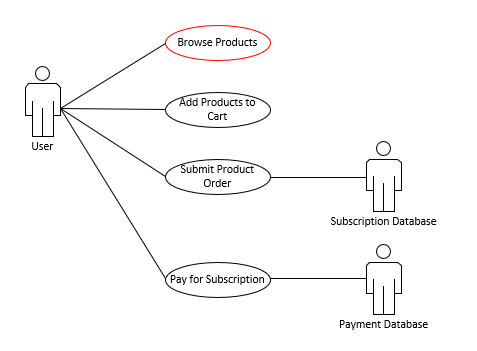
\includegraphics[scale=0.5]{UseCaseDiagrams}
	\item System Workflows using \textbf{Activity Diagrams}
	\newline
	Activity diagrams show how the system will accomplish the requirements set out in the user case diagrams. High-level actions are linked together to represent a process that needs to occur in the system \cite{Lamport:UML}.
	\newline
	The figure below shows an activity diagram from our class project.
	\newline
	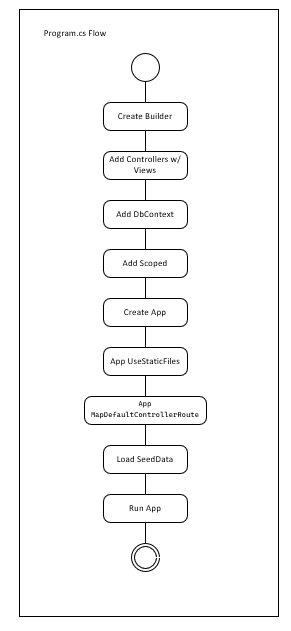
\includegraphics[scale=0.5]{ActivityDiagram}
	\item A Systems Logical Structure using \textbf{Class Diagrams}
	\newline
	Class diagrams show classes and their relationships \cite{Lamport:UML}.
	\newline
	The figure below shows a class diagram from our class project.
	\newline
	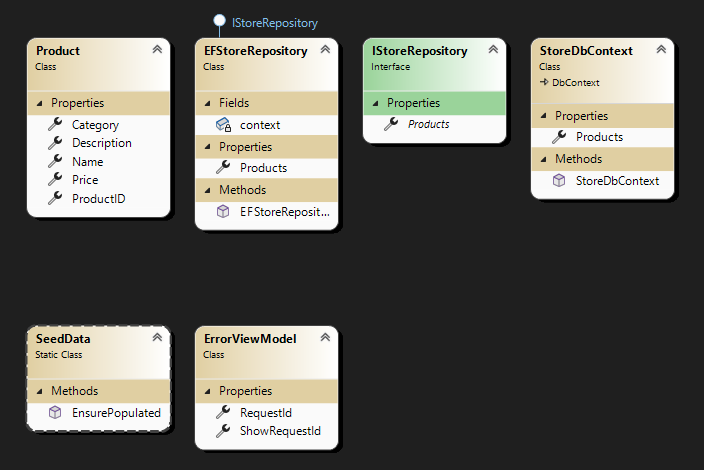
\includegraphics[scale=0.4]{ClassDiagrams}
	\item Ordered Interactions using \textbf{Sequence Diagrams}
	\newline
	Sequence diagrams are an important member of a group known as interaction diagrams. They help accurately model how the parts that make up the system interact.  They capture the order of interactions between parts of the system, describe which interactions will be triggered and in what order those interactions will occur \cite{Lamport:UML}.
	\newline
	The figure below shows a sequence diagram from our class project.
	\newline
	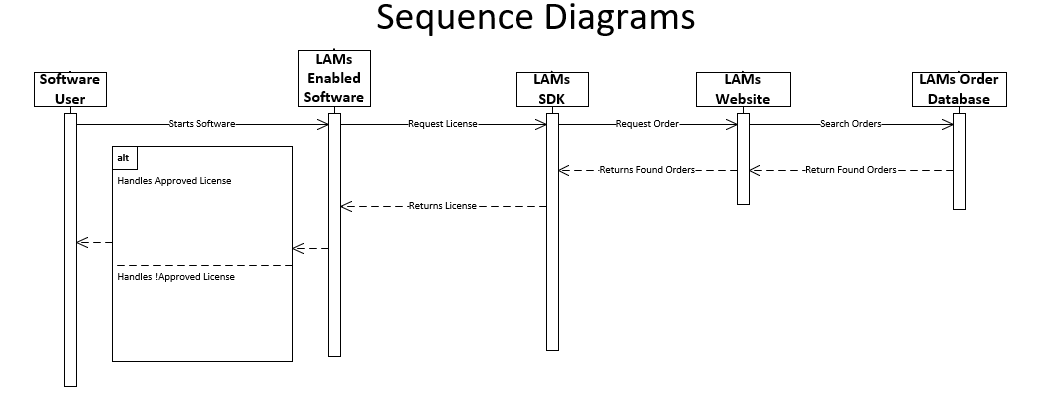
\includegraphics[scale=0.3]{SequenceDiagram}
	\item Interaction Links using \textbf{Communication Diagrams}
	\newline
	Communication Diagrams are also a member of the group known as interaction diagrams. They focus on the links between participants and are good at showing which links are needed to pass messages. They also show the links between participants that are required for events that make up the interaction \cite{Lamport:UML}.
	\item Interaction Timing using \textbf{Timing Diagrams} 
	\newline
	Timing Diagrams are all about timing to model detailed timing information. These kinds of diagrams are mostly associated with real time and embedded systems, but may also be applied to other types of systems. Each event has the following information associated with it: when the event was invoked, how long it takes for another participant to receive the event, and how long the receiver will be in that particular state \cite{Lamport:UML}.
	\item Interaction Picture using \textbf{Interaction Overview Diagrams}
	\newline
	Interaction Overview Diagrams combine sequence diagrams, communication diagrams, and timing diagrams to show the higher-level picture. They result in having a better feel for what you are doing and the context in which you are doing it. Each part of an interaction overview is a complete interaction in itself. This diagram glues together the components in a way that makes the most sense to show how things work together \cite{Lamport:UML}.
	\item Internal Class Structure using \textbf{Composite Structures}
	\newline
	Composite Structures are part of the Logical View of your system. They come in handy when class or sequence diagrams don't quite work. These diagrams are relatively advanced in nature are are suited for situations such as internal structures which show the parts contained by a class, ports, and collaborations which show design patterns and how objects cooperate to meet a requirement \cite{Lamport:UML}.
	\item System Parts using \textbf{Component Diagrams}
	\newline
	Component Diagrams are part of the Development View which show how your system is organized into modules and components. This helps to manage layers within your systems architecture. Component Diagrams also help you manage complexities and dependencies between the parts. A component is an encapsulated, reusable, and replaceable part of your system which acts like a building block which can be combined into even larger component building blocks \cite{Lamport:UML}.
	\item Organize Your Model using \textbf{Packages}
	\newline
	Packages are part of the Development View and are used to group like UML elements together. In the case of grouping classes, namespaces are used. Namespaces are typically folders that contain like objects. For example, a folder named Models may be created to contain all classes that are model object classes. Packages help keep things organized. Also, dependencies between packages can be shown, which is an important fact to know \cite{Lamport:UML}.
	\item Object State using \textbf{State Machine Diagrams}
	\newline
	State Machine Diagrams are part of the Logical View and are used to show the state of objects and the events that trigger the objects to change state. A state diagram consists of states, transitions, and events. A transition represents a change of state or how to get from one state to another. The event is was causes the transition. A state becomes active when it is entered and inactive when it is exited. State diagrams are used frequently in real-time, mission critical applications, dedicated devices, and in games \cite{Lamport:UML}.
	\newline
	The figure below shows a state diagram from \cite{Lamport:UML}.
	\newline
	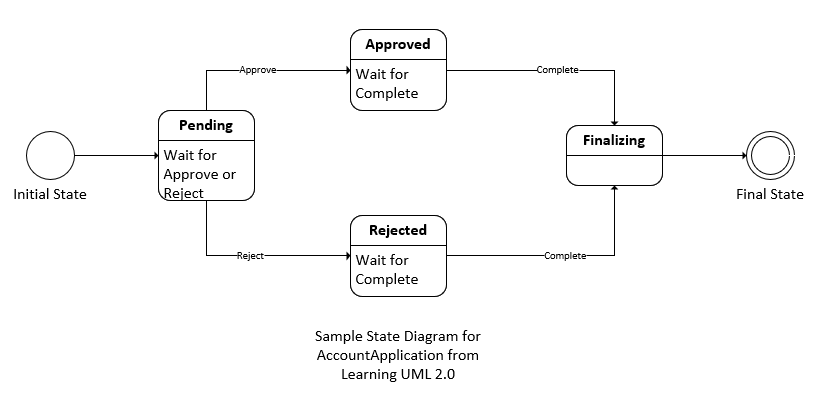
\includegraphics[scale=0.3]{StateDiagrams}
	\item The Deployed System using \textbf{Deployment Diagrams}
	\newline
	Deployment Diagrams are part of the Physical View and show both the hardware and software components of the system and how they are deployed. This view is especially helpful to stakeholders to show them how the final delivered system will look. In these diagrams, hardware is referred to as a node and software is referred to as an artifact. These diagrams evolve over the lifetime of the project and contain enough information to support the systems needs \cite{Lamport:UML}.
\end{enumerate}
A picture is worth 1024 words! The title of chapter 12 in Software Requirements. Wiegers and Beatty discuss the importance of using both textual and visual representations at different levels of abstraction to capture the full intentions of the intended system \cite{Lamport:SoftwareRequirements}. "Comparing the different representations of requirements reveals inconsistencies, ambiguities, assumptions, and omissions that would otherwise be difficult to spot" \cite{Lamport:SoftwareRequirements}. The authors stress that visual representations should augment and not replace natural language specifications \cite{Lamport:SoftwareRequirements}.

Their book describes the following visual requirements models \cite{Lamport:SoftwareRequirements}.
\begin{enumerate}
	\item Data flow diagrams (DFDs)
	
	\item Process flow diagrams 
	\item State-transition diagrams and state tables
	\item Dialog maps
	\item Decision tables and decision trees
	\item Event-response tables
	\item Feature trees (Ch 5)
	\item Use case diagrams (Ch 8)
	\item Activity diagrams (Ch 8)
	\item Entity-relationship diagrams (Ch 13)
\end{enumerate}
Wiegers and Beatty also briefly discuss the use of visual models in agile driven projects \cite{Lamport:SoftwareRequirements}.

Weilkiens introduces a toolbox that can be used for modeling complex and distributed systems called SYSMOD. This toolbox helps to alleviate some of the problems due to rising complexity of systems. There is a great need to express component systems in a way that can be easily shared between team members. A shared language is important for being able to complete the design task \cite{Lamport:SysML}.

The American Institute of Architects discuss the need for standard content and graphics to be used by Construction Architects to document their projects (Appendix E). \cite{Lamport:AIA_Graphical_Standards}. Although software architecture and construction architecture are technically different fields, they share many common goals of turning stakeholder ideas into a real products.
\newline
The US CAD Standard (NCS) is a compilation of related documents published by several organizations for the purposes of creating a national standard for construction related CAD documents. \cite{Lamport:AIA_Graphical_Standards}.\newline
A national CAD standard provides the following advantages \cite{Lamport:AIA_Graphical_Standards}
\begin{enumerate}
	\item Allows information to be transfered throughout the project cycle from one professional to another.
	\item Results in better coordination between architects and engineers
	\item Saves production time
	\item Improves the overall design of the project
\end{enumerate}
The Uniform Drawing System consist of 8 modules that help standardize the documents needed to convey information from the architect to the builder \cite{Lamport:AIA_Graphical_Standards}.
\begin{enumerate}
	\item Module 1 - Drawing Set Organization
	\item Module 2 - Sheet Organization
	\item Module 3 - Schedules
	\item Module 4 - Drafting Conventions
	\item Module 5 - Terms and Abbreviations
	\item Module 6 - Symbols
	\item Module 7 - Notations
	\item Module 8 - Code Conventions
\end{enumerate}

Of particular interest is the recommendation of using of a drawing set hierarchy in the NCS.  

Ingeno discusses methods for documenting and reviewing software architectures \cite{Lamport:SoftwareArchitectureHandbook} In particular, he discusses
\begin{enumerate}
	\item Uses of software architecture documentation
	\item Creating architecture descriptions (ADs), including architecture views
	\item Using UML to document software architecture
	\item Reviewing software architecture documents
\end{enumerate}

Other work that is somewhat related to Software Architecture documentation can be found by searching for articles related to Construction Architecture documentation. By replacing the verb construction with the verb software development, replacing the noun building with the noun application and replacing the noun material(s) with class or instance in these articles, one will see the striking resemblence between Software Architecture and Construction Architecture. One such article I found interesting can be found here
\href{https://pinnacleinfotech.com/importance-of-detailed-architectural-drawings-in-modern-construction/}{The Importance of Detailed Architectural Drawings in Modern Construction, Pinnacle Infotech, 2024}
\newline
\newline
Bobek and Tversky presented a paper on how learning can be improved by using visuals \cite{Lamport:VisualExplanations}. They state that "creating visual explanations is superior to creating verbal ones. There are several notable differences between visual and verbal explanations; visual explanations map thought more directly than words and provide checks for completeness and coherence as well as a platform for inference, notably from structure to process." \cite{Lamport:VisualExplanations}

\section{Proposed Approach}
A table will be generated showing which format is recommended by each professional or professional association.

\section{Experimental Results}
Table 1 summarizes the opinions of various experts in the field of technical documentation.
\begin{table}[ht]
	\caption{Expert Recommendations for Document Formats} % title of Table
	\centering % used for centering table
	\begin{tabular}{c c c c} % centered columns (4 columns)
		\hline\hline %inserts double horizontal lines
		Expert & Text & Graphics & Both \\ [0.5ex] % inserts table
		%heading
		\hline % inserts single horizontal line
		Miles and Hamilton \cite{Lamport:UML} &  &  & Yes \\ % inserting body of the table
		Wiegers and Beatty \cite{Lamport:SoftwareRequirements} &  &  & Yes \\
		Weilkiens \cite{Lamport:SysML} &  &  & Yes \\
		Ingeno \cite{Lamport:SoftwareArchitectureHandbook} &  &  & Yes \\
		Lamsweerde \cite{Lamport:RequirementsEngineering} &  &  & Yes \\
		AIA \cite{Lamport:AIA_Graphical_Standards} &  &  & Yes \\
		NCS \cite{Lamport:NCS} &  &  & Yes \\ [1ex] % [1ex] adds vertical space
		\hline %inserts single line
	\end{tabular}
	\label{table:nonlin} % is used to refer this table in the text
\end{table}

\section{Discussion}
Table 1 shows that the majority of leading experts in software documentation agree that graphics, in conjunction with text, enhance the accuracy, completeness, and comprehensibility of software documents. It is encouraging to see current curriculum is CS studies including training on the use of UML diagrams in software documentation. The software industry would benefit from pushing this concept further by defining detailed drawing standards for using UML diagrams and other modeling techniques as is found in the NCS (National CAD Standard) papers and the AIA Standards for Graphics. For example, the creation of a National CAD Standard for Software Architecture (NCSSA) that mirrors the thoroughness of the NCS would be a good start. We must be aware that the creation of such a standard would take many years and require the input and buyin of many industry leaders to be successful.

\section{Threats to Validity}
When we evaluate our findings while writing this paper, which explores the effectiveness or using both textual and graphical formats to improve communication between software architects and developers, we must acknowledge the limitations.
\newline
One challenge that this paper faces is the ambiguity of the definitions of "textual" and "graphical" documentation formats. Our study assumes that textual involves written natural language while graphical formats include diagrams such as UML that have been shown in this paper. However, Weigers and Beatty say that the integration of text and visuals is subject to varying interpretations, which can lead to inconsistent applications in real-world scenarios. \cite{Lamport:SoftwareRequirements}
\newline
The recommendations provided are based on existing literature which can include bias when selecting the sources. If all relevant works were not included in the studies, then it could limit the breadth of insight. The evaluation of diagrams in graphical format is subjective which means that different researchers may assess them based on their own individual experiences and project contexts.
\newline
The generalization of the findings could be limited due to individual basis in general software practices. The conclusions may not apply equally to all types of software projects, more specifically those specified in domains such as embedded systems, real-time systems, or exploratory research projects. Furthermore, the research does not account for the rapid evolution of documentation tools and their influence to the effectiveness of either text-based or graphical formats.
\newline
Some limitations of our study is that some of the conclusions come from existing literature and expert insight. This approach provides a foundation for understanding the topic but conducting new studies with direct observations or experiments would strengthen these findings.
\newline
\newline

\section{Conclusions and Future Work}
Because natural language specifications can result in incomplete and/or inaccurate application builds, natural language only specifications should be limited to very few circumstances. Due to the fact that most applications need to both evolve over time and will eventually require maintenance, our conclusion is that the majority of software specifications need to include both natural language and graphical representations to fully document their functionality. This will lead to more complete and accurate implementation of specifications by software developers.
\newline
There are several opportunities for future work regarding software documentation. Here is a list of a few that we thought of.
\begin{enumerate}
	\item Perform controlled studies were one group of software developers is given documents with text only and another group is given the same documents but are augmented with diagrams and graphics. Compare the results to see if there is a significant difference.
	\item Examine CAD standards and determine how they may be applicable to software development documentation.
	\item Examine software project failures and determine which percentage of those projects used documentation that included detailed diagrams. 
\end{enumerate}

\section{Acknowledgments}
We would like to thank Dr. Kristen Walcott, Dr. Armin Moin and the Computer Science and Software Engineering Department at UCCS for helping us gain a deeper understanding of the challenges and opportunities in software architecture.

 
%
% The following two commands are all you need in the
% initial runs of your .tex file to
% produce the bibliography for the citations in your paper.
\bibliographystyle{abbrv}
\bibliography{sigproc}  % sigproc.bib is the name of the Bibliography in this case
% You must have a proper ".bib" file
%  and remember to run:
% latex bibtex latex latex
% to resolve all references
%
% ACM needs 'a single self-contained file'!
%

\balancecolumns
% That's all folks!
\end{document}
